%%%%%%%%%%%%%%%%%%%%%%%%%%%%%%%%%%%%%%%%%
% Simple Sectioned Essay Template
% LaTeX Template
%
% This template has been downloaded from:
% http://www.latextemplates.com
%
% Note:
% The \lipsum[#] commands throughout this template generate dummy text
% to fill the template out. These commands should all be removed when 
% writing essay content.
%
%%%%%%%%%%%%%%%%%%%%%%%%%%%%%%%%%%%%%%%%%

%----------------------------------------------------------------------------------------
%	PACKAGES AND OTHER DOCUMENT CONFIGURATIONS
%----------------------------------------------------------------------------------------

\documentclass[12pt]{article} % Default font size is 12pt, it can be changed here

%\usepackage{geometry} % Required to change the page size to A4
%\geometry{a4paper} % Set the page size to be A4 as opposed to the default US Letter

\usepackage{graphicx} % Required for including pictures

\usepackage{float} % Allows putting an [H] in \begin{figure} to specify the exact location of the figure
\usepackage{wrapfig} % Allows in-line images such as the example fish picture

\usepackage{lipsum} % Used for inserting dummy 'Lorem ipsum' text into the template
\usepackage{xfrac}
\linespread{1.2} % Line spacing

%\setlength\parindent{0pt} % Uncomment to remove all indentation from paragraphs

\graphicspath{{Pictures/}} % Specifies the directory where pictures are stored

\usepackage{url}
\usepackage{bm}
\usepackage{bbm}
\usepackage{sidecap}
\usepackage{listings}
\usepackage[dvipsnames]{xcolor}
\newcommand{\sign}{\text{sign}}
\usepackage{courier}
\usepackage{algorithm, algpseudocode}
\usepackage{wrapfig}
\usepackage[font=small, labelfont=bf]{caption}
\usepackage{hyperref}
\usepackage[dvipdfmx]{animate}
\hypersetup{% hyperref Option list
setpagesize=false,
 bookmarksnumbered=true,%
 bookmarksopen=true,%
 colorlinks=true,%
 linkcolor=blue,
 citecolor=red,
}

\begin{document}

%----------------------------------------------------------------------------------------
%	TITLE PAGE
%----------------------------------------------------------------------------------------

\begin{titlepage}

\newcommand{\HRule}{\rule{\linewidth}{0.5mm}} % Defines a new command for the horizontal lines, change thickness here

\center % Center everything on the page

%\textsc{\LARGE Columbia University}\\[1.5cm] % Name of your university/college
%\textsc{\Large School of Engineering and Applied Science}\\[0.5cm] % Major heading such as course name
%\textsc{\large Mechanical Engineering}\\[0.5cm] % Minor heading such as course title

\HRule \\[0.4cm]
{ \huge \bfseries Co-Evolutionary Algorithms for Motion Planning of Multiple Manipulators}\\ [0.4cm] % Title of your document
\HRule \\[1.5cm]

%\begin{minipage}{0.4\textwidth}
%\begin{flushleft} \large
%\emph{Author:}\\
%Junji Hanatani \textsc{Smith} % Your name
%\end{flushleft}
%\end{minipage}
%~
%\begin{minipage}{0.4\textwidth}
%\begin{flushright} \large
%\emph{Supervisor:} \\
%Prof. Hod Lipson \textsc{Smith} % Supervisor's Name
%\end{flushright}
%\end{minipage}\\[4cm]

{\large \today}\\[3cm] % Date, change the \today to a set date if you want to be precise

%\includegraphics{Logo}\\[1cm] % Include a department/university logo - this will require the graphicx package

\vfill % Fill the rest of the page with whitespace

\end{titlepage}

%----------------------------------------------------------------------------------------
%	TABLE OF CONTENTS
%----------------------------------------------------------------------------------------

\tableofcontents % Include a table of contents

\newpage % Begins the essay on a new page instead of on the same page as the table of contents 

%----------------------------------------------------------------------------------------
%	INTRODUCTION
%----------------------------------------------------------------------------------------

\section{Introduction} % Major section

Robots are making our society more automated, starting from factories to our home and offices. As we expand the use of robots and increase the variations of the robot designs, the motion planning problem for the robots becomes a more significant challenge in robotics field. Over the last decades, engineers have been required to program robotic motion manually for a specific robot and a specific task, and the effort must be repeated every time the environment changes. This time-consuming process will put a limit on potential growth of the robotic products and services unless the researchers develop technique that can automatically generate all required robotic motions for the variety of tasks.

This study deals with the problem of motion planning for multiple robot arms sharing a common workspace. Multiple robots in such a setup can be used to facilitate various operations. For example, the handling operations of flexible material can be more efficiently carried out using more than one manipulators. While multiple cooperating robots can have remarkable benefits, it is more difficult to address the motion planning problem for these robots because the collision immediately happens if one robot does not take into account the motion of the other one. The simplest way to deal with this problem is defining the safety area for one robot and the other robot never enters that area. Another common approach is that one robot constantly tracks the position of the other robot and generates its motions so that no collision occurs. The motions generated by these approaches, however, limits the performance of the robots because of lack of synergy.

In this paper, we formulate this problem as an optimization problem and solve it using a method based on Genetic Algorithms \cite{Holland},\cite{David}, which minimize costs associated with a traveling length and the number of collisions. Our goal is to explore the methods of GA capable to generate well synthesized multiple robots motion more efficiently than conventional GAs. This paper is organized as follows: In Section 2, we review some related works. In Section 3, the problem is formulated and the details of proposed GA are discussed. The results of our experiments are reported in Section 4. The last section concludes the paper.

%\begin{figure}[H] % Example image
%\center{
\includegraphics[width=0.5\linewidth]{placeholder}}
%\caption{Example image.}
%\label{fig:speciation}
%\end{figure}

%\newpage
%----------------------------------------------------------------------------------------
%	Related works
%----------------------------------------------------------------------------------------

\section{Related works} % Major section

\subsection{Motion Planning}
Motion planning is responsible to finding a kinematic sequence from a start configuration to a goal configuration of the robot without touching any obstacles. To reduce the complexity of the problem, we generally consider this problem in a configuration space (C-space)\cite{Lozano} instead of the physical space where robots and obstacles exist. This turns the motion planning problem into the problem that finds a connected sequence of points $[\bm{q_{t_0}}, \bm{q_{t_1}}, \cdots ,\bm{q_{t_f}}]$, where $\bm{q_{t_0}} \in R^n$ and $\bm{q_{t_f}}\in R^n$ are the initial and goal configuration of the robot. Each via-point in the path is denoted as a vector $\bm{q_{i}}=[q_0, q_1, \cdots ,q_{n}] \in R^n$, where $n$ is the number of degree of freedom (DOF) of the robot. For example, for a 2R robot, the configuration at time $t_i$ is denoted as $\bm{q_{t_i}} = [q_{i0}, q_{i1}]$, where $q_{i0}$ is the angle of the first joint and $q_{i1}$ is the angle of the second joint (Fig.\ref{fig:C-space}).  

\begin{figure}[H] % Example image
\center{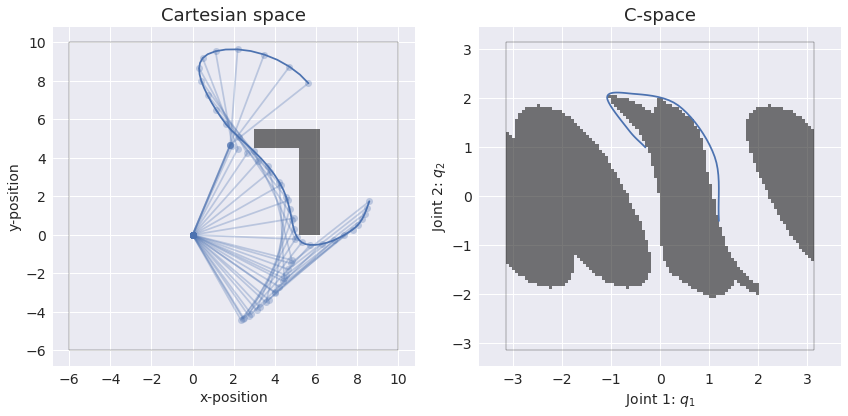
\includegraphics[width=0.75 \linewidth]{cspace}}
\caption{In the left figure, a blue line and a gray object represent a robot configuration in each time step and an obstacle in a Cartesian space respectively. In the right figure, the robot path and the object are mapped in a C-space.}
\label{fig:C-space}
\end{figure}

Many important algorithms for motion planning in a C-space fall in the category of graph search algorithms. A graph is a set of nodes connected by edges, where each edge has an associated cost such as a traveling distance. There are some general approaches to create a graph such as visibility graph\cite{Lozano2}, voronoi diagrams\cite{Aurenhammer}, cell decomposition\cite{LaValle}, or simply a grid-based map. Once discretizing the C-space and turning it into a “graph”,  graph search algorithms such as Dijkstra\cite{Cormen} or A* algorithms\cite{Zeng} ensure to find the optimal path in a discretized space. Thus, these algorithms give us the reasonable solution if the C-space is sufficiently finely discretized. \\

The main drawback of the graph search algorithms in a discretized C-space is, however, that the computational cost exponentially increases as the dimensionality of the configuration space increases. For example, the motion planning for a 7-DOF robot arm requires $10^{12}$ points if representing its C-space with grids for a resolution of 100 point per dimension, which is no longer practical. \\

Sampling-based planning such as Probabilistic Roadmap (PRM)\cite{Kavraki} or Rapidly-exploring Random Tree (RRT)\cite{LaValle2} is one of the most practical approaches for exploring the high dimensional C-space. These algorithm does not search a C-space orderly but samples random points, resulting in a relatively small number of points to be explored. These algorithms produces feasible path in a practical execution time. However, they are not guaranteed to find the optimal path. 

\subsection{Evolutinary Planner}
Genetic Algorithm\cite{Holland},\cite{David} is a method for solving an optimization problem inspired by the process of natural selection. In the context discussed in the previous section, GAs have received a lot of attention from researchers for the following reasons:

\begin{itemize}
\item The motion planning problem is known as NP-complete\cite{Canny}, meaning that the complexity of the problem grows exponentially as the number of DOF increases and it is no longer realistic to find the exact solution with deterministic algorithm.
\item Genetic Algorithms are classified as a global heuristics search. They are designed to find correct solutions that are not necessarily the best solutions as effectively as possible. 
\item Genetic Algorithms are well adapted to search for solutions in high dimensionality search space.
\item Genetic algorithms can easily be implemented on parallel machines and achieve speed up linearly with the number of processors.
\end{itemize}

The idea of the GA for the robot motion planning is introduced by Davidor\cite{Davidor} in 1991. Ahuactzin\cite{Ahuactzin} also demonstrates the path planner for both a 2-DOF robot arm and an holonomic mobile robot. Since then, many researchers have contributed to the development of both genetic encoders and genetic operators that are designed to be suitable for the motion planning problems \cite{Tian},\cite{Kazem},\cite{Macros},\cite{Macros2}.\\

GA for motion planning of the dual-arm robots are proposed by Rana and Zalzala\cite{Rana} in 1997. In their paper, paths of two robots are encoded as strings of via-points and combined into a single chromosome. Venegas and Marcial-Romero\cite{Venegas} used the decoupled approach to obtain a plan for the multiple manipulators. The strategy is to combine the exploration of the free collision space and the exploration of the target position from previously explored area. Both solutions are obtained by GA. Curkovic and Jervic\cite{Curkovic} evolves the paths for two robots based on Cooperative Coevolution in 2010. The main difference of their work from the others is that they encode the paths of robots as two separate chromosomes and evolve them among separate populations. The communication between two populations take place only when checking for collisions. Each individual is evaluated with a set of the top 10\% collaborators from the other population.

%\newpage
%----------------------------------------------------------------------------------------
%	Methods
%----------------------------------------------------------------------------------------
\section{Methods}

\subsection{Problem formulation}
Two 2R robots in a 2D space are considered first. The robot arms in the cartesian space are shown in Fig.\ref{fig:cartesian}. The first robot appears as an obstacle for the second robot and vice versa, but no obstacle exists except the robots. 

\begin{figure}[H] % Example image
\center{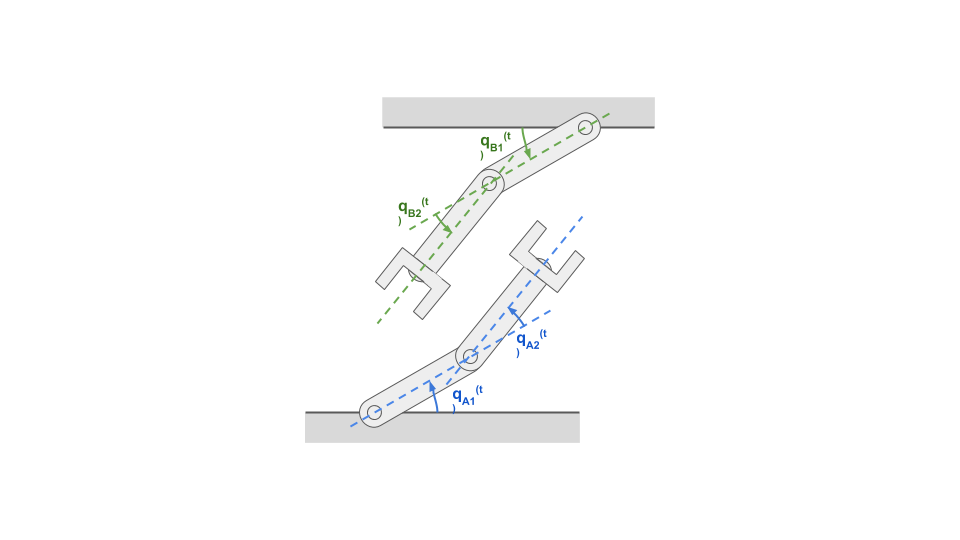
\includegraphics[width=1.0\linewidth]{2Rrobot}}
\caption{2D cartesian space for two 2R robots with two links}
\label{fig:cartesian}
\end{figure}

A configuration of the robot A at the time $t$ is denoted by $\bm{q_A^{(t)}}=[q_{A0}^{(t)}, q_{A1}^{(t)}]$ and robot B at the time $t$ is denoted by $\bm{q_B^{(t)}}=[q_{B0}^{(t)}, q_{B1}^{(t)}]$. The paths for the robot A and the robot B are represented by connecting a set of points in the C-space:
\begin{eqnarray}
\left\{ \bm{q_A^{(t_0)}} , \bm{q_A^{(t_1)}}, \cdots , \bm{q_A^{(t_f)}} \right\}\\ 
\left\{ \bm{q_B^{(t_0)}} , \bm{q_B^{(t_1)}}, \cdots , \bm{q_B^{(t_f)}} \right\}
\end{eqnarray}
,where start point $\vec{q_A^{(t_0)}}$, $\vec{q_B^{(t_0)}}$ and end point $\vec{q_A^{(t_f)}}$, $\vec{q_B^{(t_f)}}$ are given. The purpose of the motion planning is to find the set of via-points that moves the robot from start to goal as fast as possible. Geometrically, this seems to be achieved with the shortest path obtained by connecting each via-point with a line segment. However, such a path is never feasible in practice because real robots with finite acceleration cannot go through the discontinuous point of the path. The real robots require at least continuous velocity profiles. For this reason, we formulate the parametric curve $\bm{r}(s)$ with $s \in [0, 1]$, connecting two points $\bm{q^{(t_i)}}$ and $\bm{q^{(t_{i+1})}}$ as follows.

\begin{eqnarray}
\bm{r} = 
\left[ s^3, s^2, s^1, 1\right] 
  \left[ 
   	\begin{array}{cccc}
      2 & 1  & -1 & 1  \\
     -3 & -2 & 3  & -1 \\
      0 & 1  & 0  & 0  \\
      1 & 0  & 0  & 0  \\
    \end{array}
  \right]
  \left[ 
   	\begin{array}{cccc}
      \bm{q^{(t_i)}} \\
      \bm{v^{(t_i)}} \\
      \bm{q^{(t_{i+1})}} \\
      \bm{v^{(t_{i+1})}} \\
    \end{array}
  \right]
\end{eqnarray}
,where $\bm{v^{(t_i)}} = \frac{1}{2} \left( \bm{q^{(t_{i+1})}} - \bm{q^{(t_{i-1})}} 
\right)$ is a velocity at the time $t_i$. This curve is called Ferguson spline curve and ensures the continuous velocity profiles for the robotic motion.

\begin{figure}[H] % Example image
\center{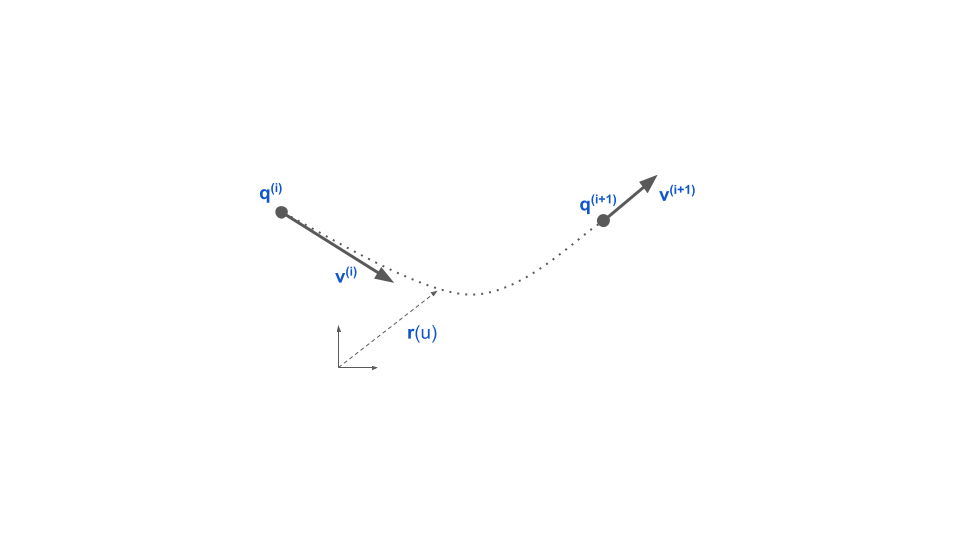
\includegraphics[width=1.0\linewidth]{spline}}
\caption{Complete robot path formulated by Ferguson spline curves.}
\label{fig:spline}
\end{figure}

%------------------------------------------------

\subsection{Co-evolutionary Genetic Algorithm} % Sub-section

\subsubsection{Representation for robot paths}

In Genetic Algorithm, the parameters to be optimized have to be encoded to a string representation. The encoding is a key process for the GA because the optimization will be successful as long as the encoded string contains compact sub-solutions of the problem (Building blocks). The solution of the motion planning problem is the entire path, which can be constructed by the combination of the sub-path segments. Thus, in that sense, it is natural that the solutions are encoded directly as strings of a sequence of the via-points as follows:
\begin{eqnarray}
\left[
\left\{ q_{A0}^{(0)}, q_{A1}^{(0)}\right\},
\left\{ q_{A0}^{(1)}, q_{A1}^{(1)}\right\},
, \cdots,
\left\{ q_{A0}^{(m-1)}, q_{A1}^{(m-1)}\right\}
\right]\\
\left[
\left\{ q_{B0}^{(0)}, q_{B1}^{(0)}\right\},
\left\{ q_{B0}^{(1)}, q_{B1}^{(1)}\right\},
, \cdots,
\left\{ q_{B0}^{(m-1)}, q_{B1}^{(m-1)}\right\}
\right]
\end{eqnarray}
In this study, the number of the via-points $m$ is set to 7. 

\subsubsection{Initial population}
At the beginning of the evolutionary process, an initial population of chromosomes is generated from scratch. This is done by selecting a random via point $\bm{q_m}$ from the C-space and connecting a given start point $\bm{q_s}$ and the via point $\bm{q_m}$, as well as the via point $\bm{q_m}$ and a given goal point $\bm{q_g}$ using the Ferguson spline curve described as Eq.(3). Then, the obtained continuous path is divided into $m-1$ sub-path segments.

\begin{figure}[H] % Example image
\center{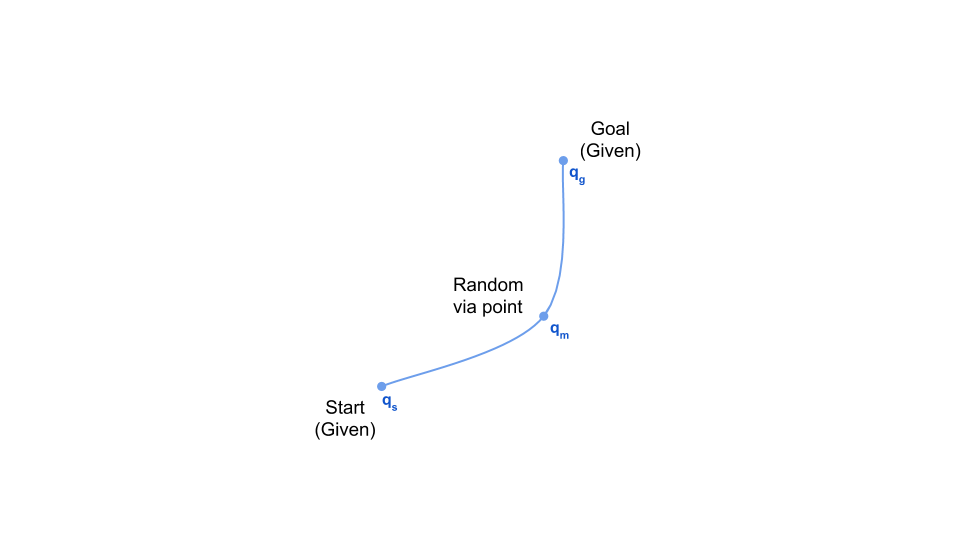
\includegraphics[width=1.0\linewidth]{initialpath}}
\caption{Random initial path.}
\label{fig:initial}
\end{figure}

\subsubsection{Genetic operators and selection mechanisms}
The progress of the evolutionary process is driven by two key process: Mutation and crossover. The purpose of mutation operators is to find a better solution around the current solution and improve the solution incrementally. Crossover operators are responsible to discovering new areas of the solution space by recombining the current solutions. Recombination of solutions are successful only when the building blocks are unlikely broken by the crossover operation. In this study, the following operators are used .

\begin{description} % Numbered list example
\item[Mutation] \hfill \\
A single point $\bm{q}$ is randomly picked from the chromosome with the probability $P_m = 0.5$, and the point is slightly shifted by adding a vector $\bm{\Delta q}$ chosen from the Gaussian distributions with mean $\mu = 0$ and variance $\sigma = 0.1$.
\end{description} 
\begin{figure}[H] % Example image
\center{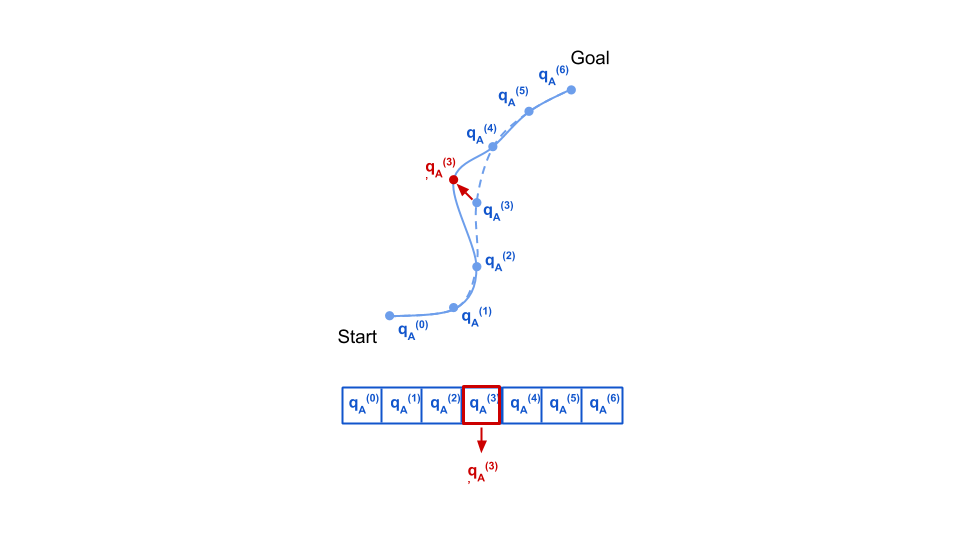
\includegraphics[width=1.0\linewidth]{mutation}}
\caption{Mutation}	
\label{fig:mutation}
\end{figure}

\begin{description}
\item[Crossover] \hfill \\
One point crossover is used. This operator is known as the conventional and simplest crossover operator for GAs, where a cut point is randomly selected from two parents chromosomes and then the tail part from the cut point are swapped between two parents. For the chromosomes encoded for the motion planning problem, however, one point crossover can degrade the quality of the path by inserting the redundant sub-path segment(Fig.\ref{fig:crossover}). To avoid this, a pair of the cut points is picked from the nearest points of the parent paths instead of the random points.
\end{description} 

\begin{figure}[H] % Example image
\center{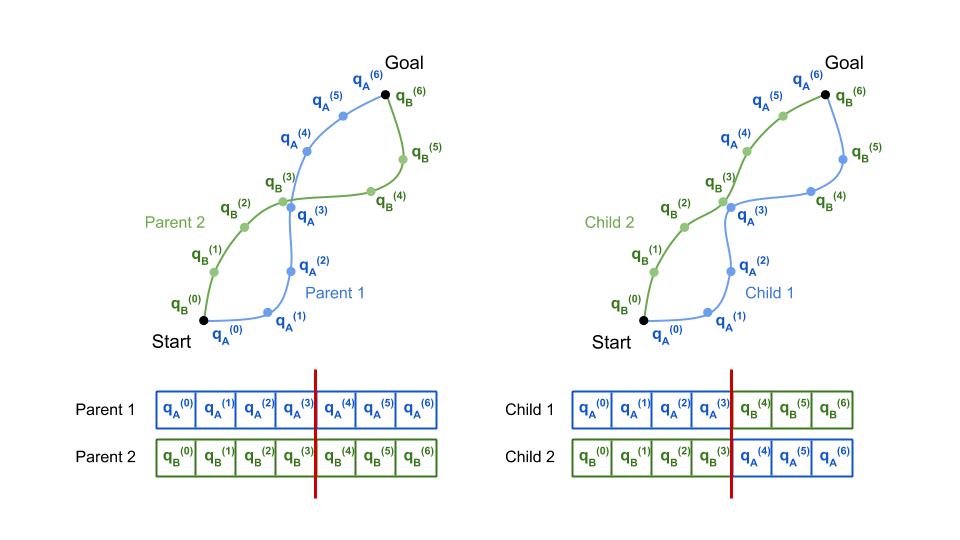
\includegraphics[width=1.0\linewidth]{crossover}}
\caption{Crossover}
\label{fig:crossover}
\end{figure}

Selection is a method for selecting individuals who will survive in the next generation and contribute to the evolution. The following selection mechanism is used in this study.

\begin{description} % Numbered list example
\item[Tournament Selection] \hfill \\
 This algorithm randomly picks up $N$ individuals from the population and creates a "tournament". The individual with the best fitness in the tournament is selected as a offspring. This tournament process is repeated until the number of offspring reaches a certain amount. The tournament size $N=3$ is used for the GA in this study.\\

\item [Elitist Selection] \hfill \\
The top $N$ individuals are selected from the population and retained in the next generation without any operation being applied. N=5 is used in this study. This selection mechanism prevents the best individuals from the destruction and guarantees that the best fitness does not decrease as the generation goes on.

\end{description} 

\subsubsection{Diversity maintenance}

To make the population more diverse, Age-Layered Population Structure (ALPS)\cite{Hornby} is introduced. The key properties of ALPS are follows: 
\begin{itemize}
\item Population are divided into the 6 age-layers. The age is measured based on how many generations the individual survives since it was born. The age limits for each layer is [5, 10, 20, 40, 80, ∞]. 
\item Every 5 generation, new population are generated from scratch and stored in the youngest layer. 
\item The next generation in the layer is selected only from the current population in the same layer. 
\item The crossover happens with individuals in the same layer or younger age layers.
\end{itemize}

\subsubsection{Subjective fitness for co-evolution}
The definition of the optimal path in this study is that, first, the number of the collision between two robots $F_c$ are as small as possible, and second, the traveling lengths of the end effector of robot A: $d_{A}$, and B: $d_{B}$ are as short as possible in a Cartesian space. In that sense, the fitness function $F$ is defined as follows:
\begin{eqnarray}
F &=& f \left( d_{A},~ d_{B} \right) + w F_c
\end{eqnarray}
, where $w$ is a weight on the fitness associated with the number of collision and set to $w=10.0$. Each component of the fitness function is described as follows:
\begin{eqnarray}
F_c &=& \sum_{k=0}^{M-1} C_k \\
C_k &=& \left\{
\begin{array}{cc}
1 & \text{if Robot A and B collide in the $k$-th configuration.}\\
0 & \text{otherwise}
\end{array}
\right.
\end{eqnarray}
Also,
\begin{eqnarray}
d_{A} &=& \sum_{k=0}^{M-1} 
\|  
\bm{p_k}     \left(\bm{q_A} \right) - 
\bm{p_{k-1}} \left(\bm{q_A} \right) 
\| \\
d_{B} &=& \sum_{k=0}^{M-1} 
\|  
\bm{p_k}     \left(\bm{q_B} \right) - 
\bm{p_{k-1}} \left(\bm{q_B} \right) 
\|
\end{eqnarray}
, where $\bm{p_k} \left(\bm{q_A} \right)$ and $\bm{p_k} \left(\bm{q_B} \right)$ are the positions of the end effector of the robot A and B in a Cartesian space at time $k$. We introduce two types of fitness functions $f \left( d_{A},~ d_{B} \right)$: Cooperative fitness and competitive fitness.
\begin{description}
\item[Cooperative fitness] \hfill \\
The robot A and B cooperate each other, i.e., the fitness value of the robot A decreases not only when the traveling length $d_A$ decreases but also the traveling length $d_B$ decreases.
\begin{eqnarray}
f \left( d_{A},~d_{B} \right) = d_{A} + d_{B} 
\end{eqnarray}
\item[Competitive fitness] \hfill \\
The robot A and B compete each other, i.e., the fitness value of the robot A decreases only when the traveling length $d_A$ decreases, but the fitness value is capped at the level of the traveling length $d_B$.
\begin{eqnarray}
f \left( d_{A},~d_{B} \right) = \max \left( d_{A} ,~ d_{B} \right) 
\end{eqnarray}
\end{description}

In this study, each fitness function is applied and compared its performance each other.
 
%\newpage
%----------------------------------------------------------------------------------------
%	Simulation results
%----------------------------------------------------------------------------------------
\section{Simulation results and discussion}
The algorithm was implemented with parameters given in Table \ref{tab:parameter}.   
% ---------------------------
\begin{table}[H]
  \begin{center}
    \caption{Parameter for Genetic Algorithm.}
    \label{tab:parameter}
    \begin{tabular}{ll} 
	\hline      
      Number of Generations          & 500  \\
      Population size in a layer    & 50   \\
      Number of points in a path    & 7 \\       
	  Number of elites              & 1 \\
	  Tournament size               & 3 \\
      Number of layers              & 5 \\
      Max age of each layer         & $ \left[ 5, 10, 20, 40, 80 \right] $\\
	  Weight on a collision fitness & 10.0 \\
	  Mutant probability            & 0.5  \\
	\hline      
    \end{tabular}
  \end{center}
 \end{table}
%----------------------------
The paths were planned with the start and end configurations given in Fig \ref{fig:startconfig}. Figure \ref{fig:cooperative} and Figure \ref{fig:competitive} shows results of the robots' motion by cooperative and competitive GA. The robots seem to overlap in each picture, but they are occurring at different time instants. Therefore collision is not occurring between them. 
  
\begin{figure}[H] % Example image
\center{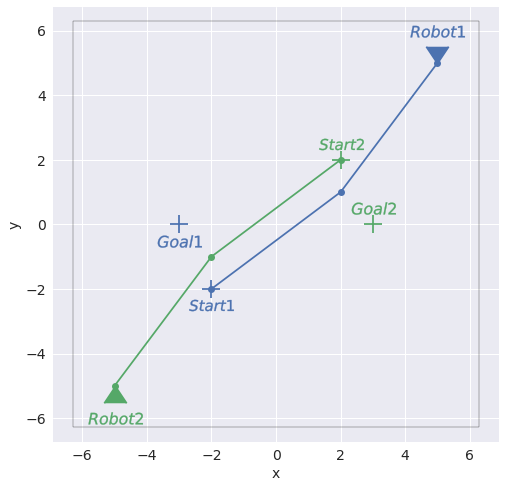
\includegraphics[width=0.4\linewidth]{configuration}}
\caption{Start configuration of the robot.}
\label{fig:startconfig}
\end{figure}

\begin{figure}[H] % Example image
\center{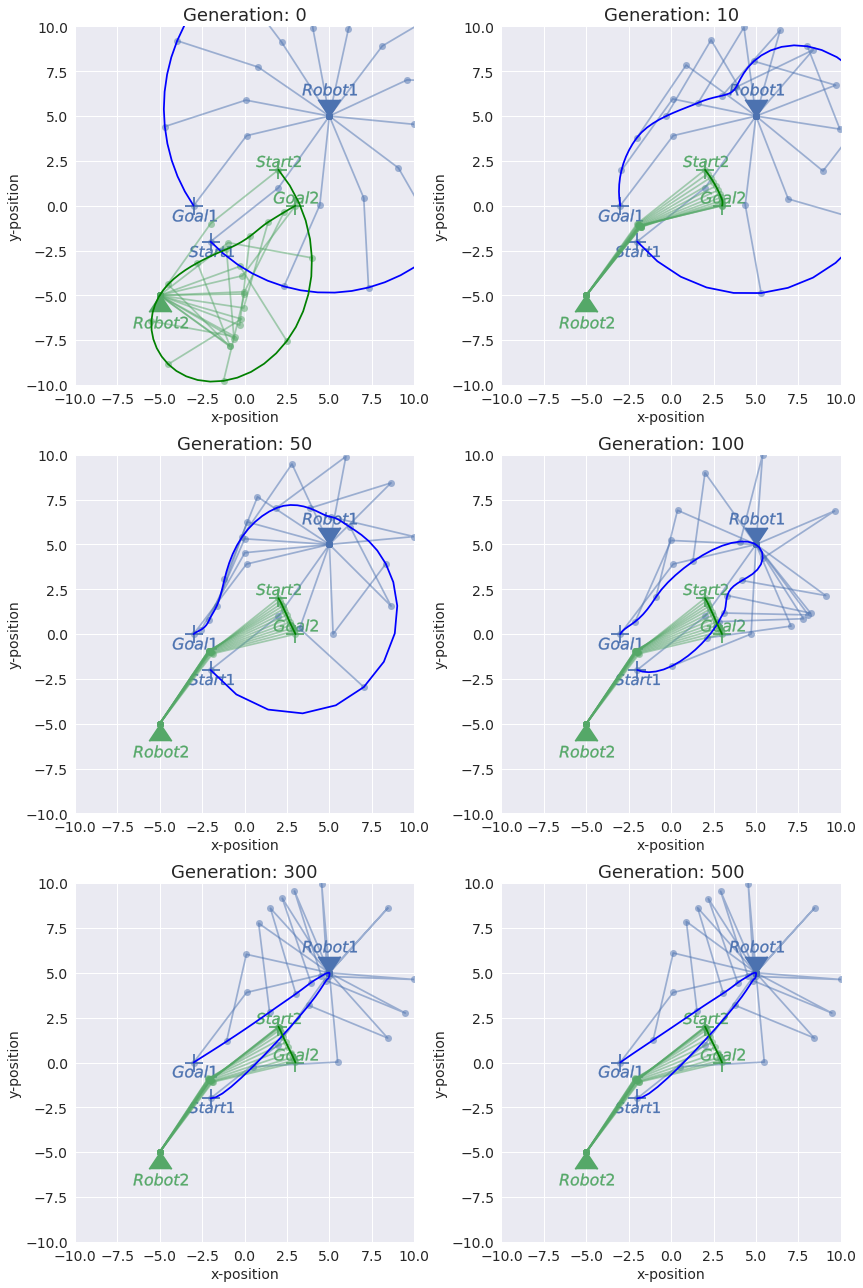
\includegraphics[width=0.9\linewidth]{cooperative2}}
\caption{The snapshot of the robot motion evolution with cooperative fitness.}
\label{fig:cooperative}
\end{figure}

\begin{figure}[H] % Example image
\center{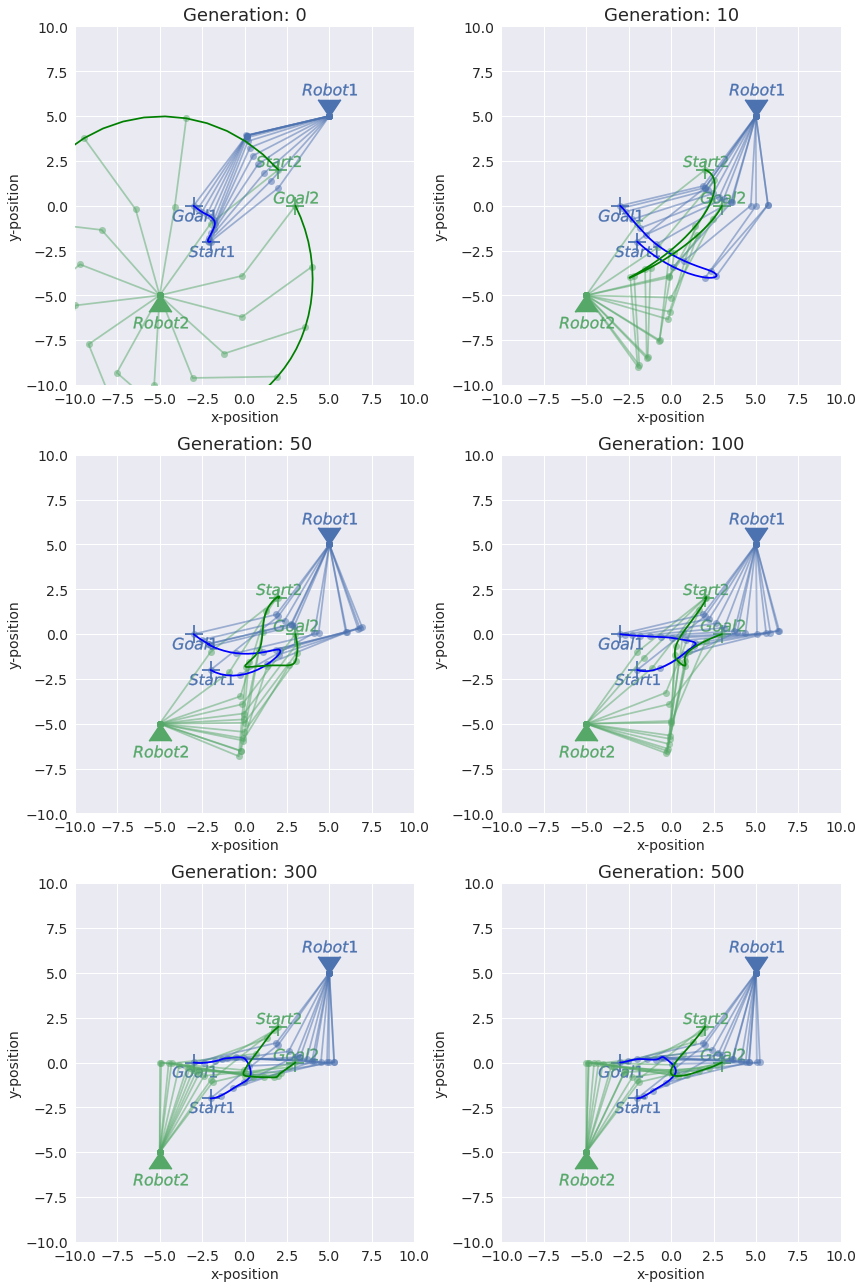
\includegraphics[width=0.9\linewidth]{competitive2}}
\caption{The snapshot of the robot motion evolution with competitive fitness}
\label{fig:competitive}
\end{figure}

The shortest path found by each planner is shown in Table \ref{tab:bestfitness}. Figure \ref{fig:learningcurve} shows The learning curve of the GA with cooperative fitness and the competitive fitness. Each is performed 5 times. The solid lines indicate the average traveling distances of the end effectors, and error bars indicate the standard error of these values. 

% ---------------------------
\begin{table}[H]
  \begin{center}
    \caption{The best paths obtained by cooperative and competitive GA.}
    \label{tab:bestfitness}
    \begin{tabular}{|l|l|l|} 
    \hline
      					          & Robot A & Robot B \\          
	\hline      
      Cooperative Co-evolution    & 2.2366  & 19.5419 \\
      Competitive Co-evolution    & 6.5236  &  6.5240 \\
	\hline      
    \end{tabular}
  \end{center}
 \end{table}
%----------------------------

\begin{figure}[H] % Example image
\center{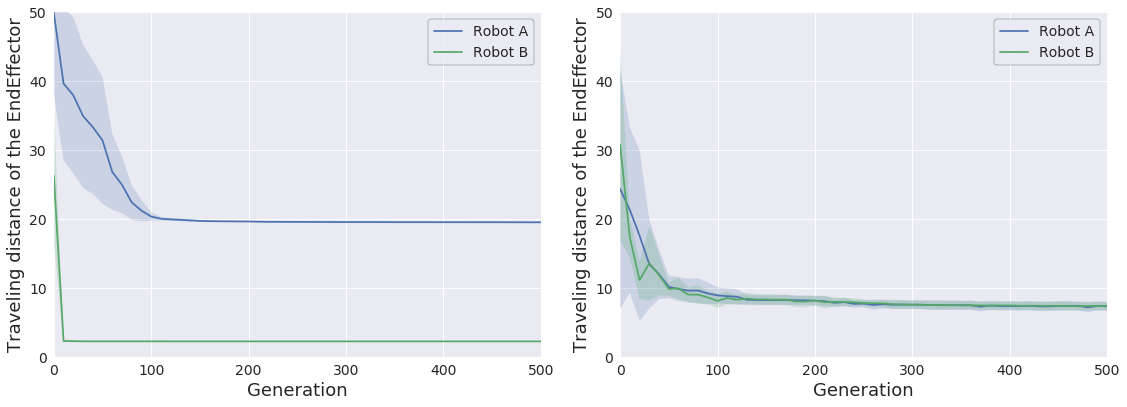
\includegraphics[width=1.0\linewidth]{Learning_curve}}
\caption{The learning curves of the evolution with cooperative fitness and competitive fitness}
\label{fig:learningcurve}
\end{figure}


In Cooperative Co-evolutionary GA, the Robot A found the path that directly leads it to the goal with the nearly shortest time. Instead of Robot A's straight forward path, the Robot B had to make a detour. On the other hand, in Competitive Co-evolutionary GA, the path lengths of both Robot A and Robot B are approximately equal. 

This difference of the multi-arm motions is obviously caused by the difference between the fitness functions of both methods. The fitness function of Cooperative Co-evolutionary GA allows one robot to obtain a good score as long as the other robot finds a short path, even if the robot itself does not find a short path. Thus, the algorithm tries to find the shortest possible path for one of the robot in exchange for the hard work of the other robot. The fitness function of Competitive Co-evolutionary GA, by contrast, makes the robots compete, which means that if the path of Robot A is shorter than that of Robot B, the Robot A stops evolving until the path of the Robot B reaches the same length as that of Robot A. As a result, both of the path length becomes nearly equal. \\

The GA with standard population structure was performed as well as GA with ALPS, and the performances are compared. The fitness curves are shown in the Figure \ref{fig:learningcurve2}. Additionally, Figure \ref{fig:dotplot} shows that the diversity of the population in each generation. \\

\begin{figure}[H] % Example image
\center{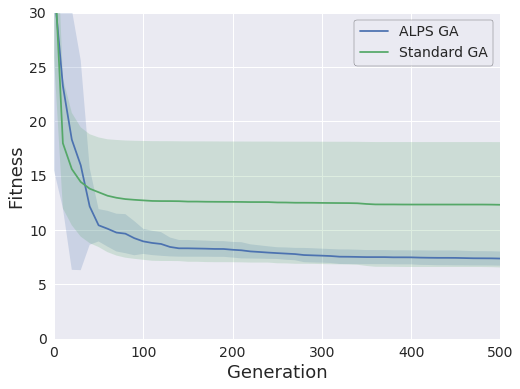
\includegraphics[width=0.5 \linewidth]{Learning_curve2}}
\caption{The learning curves of the evolution by standard GA and ALPS GA.}
\label{fig:learningcurve2}
\end{figure}

\begin{figure}[H] % Example image
\center{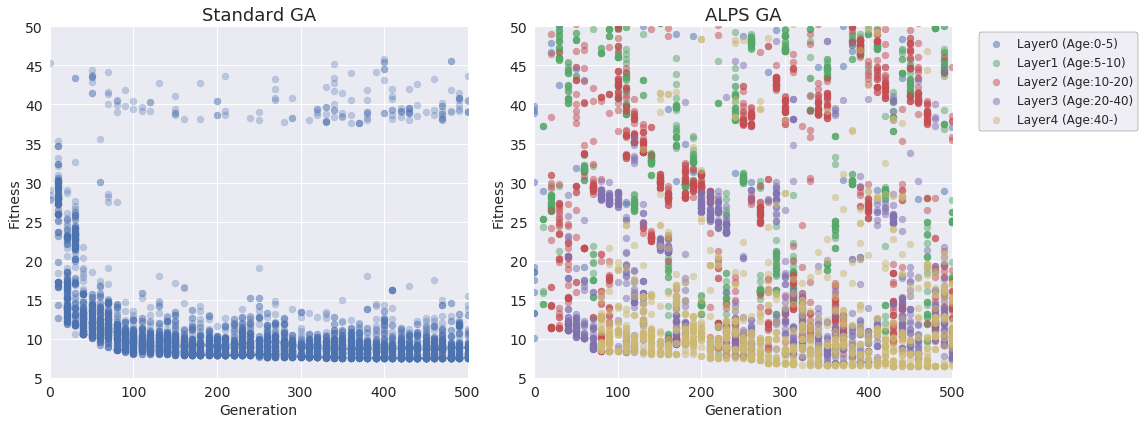
\includegraphics[width=1.0 \linewidth]{dotplot}}
\caption{Dot plot of the population with Standard GA and with ALPS GA. Each dot indicates each individual in the population.}
\label{fig:dotplot}
\end{figure}

In the Standard GA, the population lose its diversity as generation goes on, and fitness of most individuals converges into less than 15.0. By contrast, the ALPS GA successfully generates diverse population, especially in the range of fitness>15.0. As a result, it achieves better performance compared to the standard GA.

%----------------------------------------------------------------------------------------
%	Discussions
%----------------------------------------------------------------------------------------
%\section{Discussions}

%\newpage
%----------------------------------------------------------------------------------------
%	CONCLUSION
%----------------------------------------------------------------------------------------

\section{Conclusion} % Major section
In this work, we presented a new strategy for the motion planning of multi robot arms based on Co-evolutionary Genetic Algorithm. In the proposed co-evolutionary algorithm, the paths of two robots are represented as two separate populations and the fitness function for each population are dependent on the other population. We compared the performances of two types of Co-evolutionary fitnesses: competitive fitness and cooperative fitness. In the cooperative process, the sum of the both robots' traveling distances are minimized. This process generates the straight forward path connecting start and goal points directly for one robot, but the other robot has to make a detour. On the other hand, the competitive process keeps the both traveling distances balanced. As a result, in the case that the tasks for the two robots should be evenly shared, competitive process generates more natural motions.
 
This study demonstrated the proposed algorithms in the case with two 2R robots. However, considering the GA's potential to deal with high-dimensional problems, it can be adopted to the higher DOF robots and more than two robot arms. These studies need to be done in the future.	

%----------------------------------------------------------------------------------------
%\lipsum[1] % Dummy text
%\begin{wrapfigure}{l}{0.4\textwidth} % Inline image example
%  \begin{center}
%    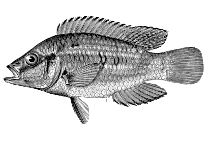
\includegraphics[width=0.38\textwidth]{fish}
%  \end{center}
%  \caption{Fish}
%\end{wrapfigure}
%\lipsum[2] % Dummy text

\newpage
%----------------------------------------------------------------------------------------
%	BIBLIOGRAPHY
%----------------------------------------------------------------------------------------

\begin{thebibliography}{99} % Bibliography - this is intentionally simple in this template

%\bibitem[1]{Figueredo:2009dg}
%Figueredo, A.~J. and Wolf, P. S.~A. (2009).
%\newblock Assortative pairing and life history strategy - a cross-cultural
%  study.
%\newblock {\em Human Nature}, 20:317--330.

\bibitem[1]{Holland}
J.H. Holland: Adaptation in Natural and Artificial Systems, Ann Arbor: University of Michigan Pres, 1975.

\bibitem[2]{David}
David E. Goldberg: Genetic algorithms in search, optimization and machine learning, The University of Alabama, Addison-Wesley publishing company, inc. 1989.

\bibitem[3]{Lozano}
Lozano-Perez, T.: Spatial planning: A configuration space approach. IEEE Trans-
actions on Computers 32(2), 108–120 (1983)

\bibitem[4]{Lozano2}
Lozano-Pérez, T.; Wesley, Michael A. (1979), "An algorithm for planning collision-free paths among polyhedral obstacles", Communications of the ACM, 22 (10): 560–570

\bibitem[5]{Aurenhammer}
Aurenhammer, Franz (1991). "Voronoi Diagrams – A Survey of a Fundamental Geometric Data Structure". ACM Computing Surveys. 23 (3): 345–405.

\bibitem[6]{LaValle} 
LaValle, Steven M (2006). "Planning Algorithms". Cambridge University Press.

\bibitem[7]{Cormen} 
Cormen, Thomas H.; Leiserson, Charles E.; Rivest, Ronald L.; Stein, Clifford (2001). "Section 24.3: Dijkstra's algorithm". Introduction to Algorithms (Second ed.). MIT Press and McGraw–Hill. pp. 595–601.

\bibitem[8]{Zeng} 
Zeng, W.; Church, R. L. (2009). "Finding shortest paths on real road networks: the case for A*". International Journal of Geographical Information Science. 23 (4): 531–543. 

\bibitem[9]{Kavraki} 
Kavraki, L. E.; Svestka, P.; Latombe, J.-C.; Overmars, M. H. (1996), "Probabilistic roadmaps for path planning in high-dimensional configuration spaces", IEEE Transactions on Robotics and Automation, 12 (4): 566–580

\bibitem[10]{LaValle2} 
LaValle, Steven M. (October 1998). "Rapidly-exploring random trees: A new tool for path planning". Technical Report. Computer Science Department, Iowa State University (TR 98-11).

\bibitem[11]{Canny}
Canny, J.: The Complexity of Robot Motion Planning. MIT Press, Boston (1988)

\bibitem[12]{Davidor}
Davidor, Y.: Genetic Algorithms and Robotics, a Heuristic Strategy for Optimization. World Scientific Publishing Co. Pte Ltd(1991).

\bibitem[13]{Ahuactzin}
Ahuactzin J.M., Talbi EG., Bessière P., Mazer E. (1993) Using genetic algorithms for robot motion planning. In: Laugier C. (eds) Geometric Reasoning for Perception and Action. GRPA 1991. Lecture Notes in Computer Science, vol 708. Springer, Berlin, Heidelberg

\bibitem[14]{Tian}
Tian, L., Collins, C. Journal of Intelligent and Robotic Systems (2003) 38: 297. 

\bibitem[15]{Kazem}
Kazem, B.I., Mahdi, A., Oudah, A.T. (2008). Motion Planning for a Robot Arm by Using Genetic Algorithm.

\bibitem[16]{Macros}
Marcos, M.D., Machado, J.A., Azevedo-Perdicoúlis, T. (2009). Trajectory planning of redundant manipulators using genetic algorithms.

\bibitem[17]{Macros2}
Marcos, M.D., Machado, J.A., Azevedo-Perdicoúlis, T. (2012). A multi-objective approach for the motion planning of redundant manipulators. Appl. Soft Comput., 12, 589-599.

\bibitem[18]{Rana}
A. S. Rana, A. M. S. Zalzala, "An evolutionary algorithm for collision free motion planning of multi-arm robots," First International Conference on Genetic Algorithms in Engineering Systems: Innovations and Applications, Sheffield, UK, 1995, pp. 123-130.

\bibitem[19]{Venegas}
Venegas, H.A., Marcial-Romero, J.R. (2009). An evolutionary algorithm for collision free motion planning of multi-arm robots. EvoWorkshops.

\bibitem[20]{Curkovic}
Curkovic, Petar. (2010). Cooperative coevolution applied to dual-arm robot motion planning. 132-137. 

\bibitem[21]{Hornby}
Hornby, G.S.: The Age-Layered Population Structure (ALPS) Evolutionary Algorithm, 


\end{thebibliography}

%----------------------------------------------------------------------------------------

\end{document}
